%!TEX program = xelatex
% 完整编译: xelatex -> bibtex -> xelatex -> xelatex

\documentclass[lang=cn,11pt,a4paper,cite=authoryear]{elegantpaper}
\usepackage{indentfirst}
\setlength{\parindent}{2em}

\title{编译原理实验一:词法分析和语法分析}
\author{林搏海}
\institute{{哈尔滨工业大学} {物联网工程}}
\date{\zhtoday}


% 本文档命令
\usepackage{array}
\newcommand{\ccr}[1]{\makecell{{\color{#1}\rule{1cm}{1cm}}}}

\begin{document}

\maketitle

\begin{abstract}
\hspace*{0.7cm}我们实现了基于Flex的词法分析和基于Bison的语法分析,构建了一颗相应的语法分析树并且将其可视化打印。在Flex语法分析中,我们实现了八进制和十六进制整型变量的识别,以及浮点数的科学计数法的识别。在构建语法分析树的过程中,我们使用了二叉树的结构来表示多叉树,并且在传参的过程中使用了C语言的变长参数函数。此外,我们采用了自底向上的过程来构建二叉树,正好对应于语法分析的LR(1)语法分析过程。
\keywords{语法分析树, 二叉树, 词法分析, Flex, Bison}
\end{abstract}



\section{词法分析}

词法分析的实现过程采用了Flex模块。基于该模块,我们只需要构造识别所有类型单词单元的正则表达式即可,Flex会将正则表达式自动生成DFA自动机程序。由于实验指导书中已经定义好了绝大部分词法单元的正则表达式,在此我们只需要生成INT, FLOAT,和ID的正则表达式即可。需要注意的是,为了方便后续对于八进制和十六进制数的转换处理,我们将八进制数和十六进制树识别为不同于十进制数INT的类型OCT和HEX。
\\ \hspace*{0.7cm} 在书写了正则表达式之后,我们需要将识别到的词法单元生成语法分析树的叶节点,方便后续完成自底向上的语法分析树的构建工作。需要注意的是,此实八进制数和十六进制数返回的叶节点类型都是INT,但是其中叶节点的value值不同,这样就可以方便后续八进制值和十六进制值转换为十进制值的处理。
\begin{figure}[h]
	\centering
	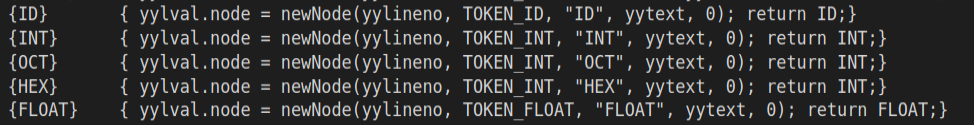
\includegraphics[width=\textwidth]{pics//1_2.png}
	\caption{叶节点生成}
\end{figure}
\\ \hspace*{0.7cm} 最后需要注意的是,我们需要对输入文本中所有的空格进行处理,将其手动忽略,同时,我们需要在正则表达书写的最后部分加上通配符'.',方便我们对错误的词法进行处理。
\begin{figure}[h]
	\centering
	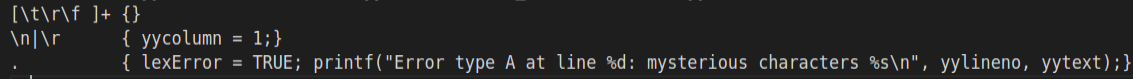
\includegraphics[width=\textwidth]{pics//1_3.png}
	\caption{空格和错误处理}
\end{figure}

\section{语法分析}
语法分析阶段的任务我们需要借助语法分析工具Bison来完成。该工具可以将我们书写的LR文法转换为对应的PDA自动机程序,由于LR文法表达式已经在实验指导书中被给出,因此,我们只需要在每一条文法的最后加入生成语法分析树节点的语义动作,并且插入error指令实现语法错误检测,最后再实现二义性文法的改造即可。
\\ \hspace*{0.7cm} 由于构造语法树的语句再词法分析和语法分析的阶段被大量使用,因此我们将其定义和是现在一个头文件中,然后我们只需要再对应的词法分析和语法分析文件中将其调用即可。在给出的LR文法中,我们发现有的父节点对应了多个子节点,因此可以考虑多叉树的实现,但是我们考虑更为简单的实现:将多叉树转换为二叉树。多叉树转换得到的二叉树的先序遍历和原本的多叉树完全相同这一性质,非常有利于我们在之后打印整个树的结构。此外,由于在构造父节点的时候,子节点的参数个数是不固定的,因此我们需要通过变长参数函数传递子节点,进行父节点的构造。
\\ \hspace*{0.7cm}在打印树结构的时候,我们只需要按照二叉树的先序遍历递归打印即可,需要注意的是由于我们使用二叉树来标识多叉树结构,因此我们需要注意在遍历树节点的时候的深度问题:根节点深度为0,访问左节点深度加一,访问右节点深度不变,然后根据传入的深度参数打印对应的空格数即可。
\\ \hspace*{0.7cm}此外,在打印语法分析树的时候,对于INT类型的树节点,我们需要关注其节点的name值,如果为HEX或者OCT,那么我们需要按照十六进制和八进制转换十进制的规则对于输出值进行转换。


在完成了对于语法分析树结构的定义和操作实现之后,我们就需要将相应的节点生成操作插入到LR语法分析的末尾,然后我们还需要谨慎的定义error的插入位置,我们需要尽可能的将error插入在较为底层的LR语法中,防止其将某些错误情况合并,造成错误的延迟发现。同时,为了使得错误分析更为清晰,我们重写了报错函数。
\begin{figure}[h]
	\centering
	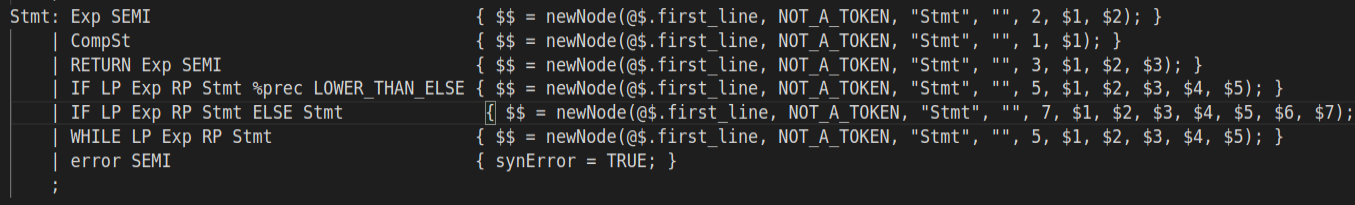
\includegraphics[width=\textwidth]{pics//2_2.png}
	\caption{语义操作}
\end{figure}
\begin{figure}[h]
	\centering
	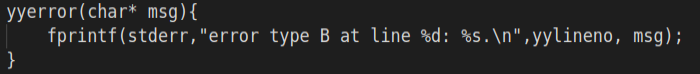
\includegraphics[width=\textwidth]{pics//2_3.png}
	\caption{错误函数}
\end{figure}
\section{主程序模块}
为了方便编译和调试,我们将main函数放在了main.c文件中,其具体逻辑入下:首先,读入我们的cmm文件,调用yyparse()函数对其进行词法分析和语法分析,如果此过程没有错误,则运行打印语法分析树的模块将程序的树结构完整输出到屏幕上,如果词法分析阶段或者是语法分析阶段检测到错误,那么我们就调用我们自己重写的error函数进行报错。
\section{编译执行方式}
程序的正确编译执行需要以下六个文件:enum.h, PTnode.h, lexical.l, main.c, syntax.y, makefile,只需要确保他们处在同一个目录下,然后执行make命令调用makefile文件执行自动编译即可。

\end{document}
